\documentclass[10pt,a4paper,ragged2e]{altacv}
\usepackage{hyperref}
\usepackage{paracol}
\usepackage{graphicx}

\geometry{left=1.25cm,right=1.25cm,top=1.5cm,bottom=1.5cm,columnsep=1.2cm}

\ifxetexorluatex
  \setmainfont{Lato}
\else
  \usepackage[utf8]{inputenc}
  \usepackage[T1]{fontenc}
  \usepackage[default]{lato}
\fi

\definecolor{VividPurple}{HTML}{3E0097}
\definecolor{SlateGrey}{HTML}{2E2E2E}
\definecolor{LightGrey}{HTML}{666666}
\colorlet{heading}{VividPurple}
\colorlet{accent}{VividPurple}
\colorlet{emphasis}{SlateGrey}
\colorlet{body}{LightGrey}

\renewcommand{\itemmarker}{{\small\textbullet}}
\renewcommand{\ratingmarker}{\faCircle}

\begin{document}
\name{Thuy Trinh Nguyen}
\tagline{Fresh Graduate in Information Systems}


%\photo{3.5cm}{images/square.jpg}
\personalinfo{
 \mailaddress{thuytrinhnguyen9@gmail.com}
 \phone{0452 280 034}
 \location{Sydney, NSW}
% \linkedin{linkedin.com/in/thuy-trinh-nguyen}
 \github{https://github.com/thuytrinhnguyen} 
}

\makecvheader

\AtBeginEnvironment{itemize}{\small}

\columnratio{0.5}

\begin{paracol}{2}

\cvsection{Education}

\cvevent{BCom - Business Information Systems}{Macquarie University}{Jul 2018 -- Jul 2020}{\href{https://www.myequals.net/sharelink/6e263be8-2699-43f9-ab57-157848d8e785/a5dd70e3-ea39-4fa8-9c9b-d8799a70afb6}{Official Transcript}}

\begin{itemize}
	\item Awarded the Macquarie University Award for Academic Excellence 2020
	\item Awarded the Qualtrics XM Research Prize - Undergraduate for Proficiency in Marketing Research unit
\end{itemize}

\switchcolumn

\cvsection{Skills}

\cvtag{Software Development} 
\cvtag{Web Development} 

\cvtag{Deep Learning} 
\cvtag{Data Analytics} 

\divider\smallskip

\cvtag{Python}
\cvtag{Java}
\cvtag{Spring}
\cvtag{Javascript}
\cvtag{React}

\cvtag{R}
\cvtag{Git}
\cvtag{Latex}

\end{paracol}

\vskip 0.1in

\columnratio{0.5}

\begin{paracol}{2}
\cvsection{Experience}

\cvevent{}{Data Analyst Part-time}{Sep 2020 - Present}{BeU AI}

\cvevent{}{Research on Reliable AI in Fake Profile Detection}{Sep 2020}{}
\begin{itemize}
	\item Research project about ... applied to CHI ...
	\item Literature review
	\item Qualitative analysis
	\subitem 
	\subitem 
	\item Techiques:
	\item Technologies:
\end{itemize}

\cvevent{}{Credit Scoring}{Oct 2020}{}
\begin{itemize}
	\item Secondary research
	\item Feature engineering
	\item 
	\subitem 
	\subitem 
	\item Technologies:
\end{itemize}

\cvevent{}{Competition on Fake News detection}{Oct 2020 - Present}{}
\begin{itemize}
	\item Data cleaning
	\item Annotation
	\item Annotator Team Lead
	\subitem 
	\subitem 
	\item Technologies: 
\end{itemize}

\cvevent{}{Lead Sales using AI and Big Data}{Nov 2020 - Present}{}
\begin{itemize}
	\item Exploratory data analysis
	\item Report
	\item Annotator Team Lead
	\item 
	\subitem 
	\subitem 
	\item Technologies: 
\end{itemize}

\switchcolumn

\cvsection{Publication}

\cvevent{Le, D. T., Vu, X. S., To, N. D., Nguyen, H. Q., Nguyen, T. T., Le, L., ... \& Nguyen, H. D. (2020). ReINTEL: A Multimodal Data Challenge for Responsible Information Identification on Social Network Sites. In Proceedings of the 7th International Workshop on Vietnamese Language and Speech Processing (pp. 84–91). Association for Computational Linguistics.}{Competition on Fake News detection}{Oct 2020 - Present}{DEF}
\begin{itemize}
	\item Data cleaning
	\item Annotation
	\item Annotator Team Lead
	\subitem 
	\subitem 
	\item Technologies: 
\end{itemize}

\cvevent{}{Nguyen, T. T., Chai, J. C., Eiring, Ø., Wang, W., O’Donnell, R. R., \& Nguyen, H. D. (2021). Gamified Mobile Health Interventions for Mental Well-being of Older Adults. International Conference on Human-Computer Interaction, 2021.}{Oct 2020 - Present}{DEF}
\begin{itemize}
	\item Data cleaning
	\item Annotation
	\item Annotator Team Lead
	\subitem 
	\subitem 
	\item Technologies: 
\end{itemize}

\end{paracol}
\cvsection{Personal Projects}

\columnratio{0.5}

\begin{paracol}{2}

\cvevent{}{Marketplace (Spring | React)}{Apr 2020}{\href{https://github.com/thuytrinhnguyen/marketplace/tree/dev}{Source on GitHub}}
\begin{itemize}
	\item An e-commerce website for technology products with fully functional backend and frontend
	\item Features:
	\subitem Authentication
	\subitem Product browsing
	\subitem User profile view
	\subitem Shopping cart
	\subitem Cart checkout
	\item Technologies: Java Spring 5 | React | PostgreSQL
\end{itemize}

\begin{figure}[htbp]
	\centerline{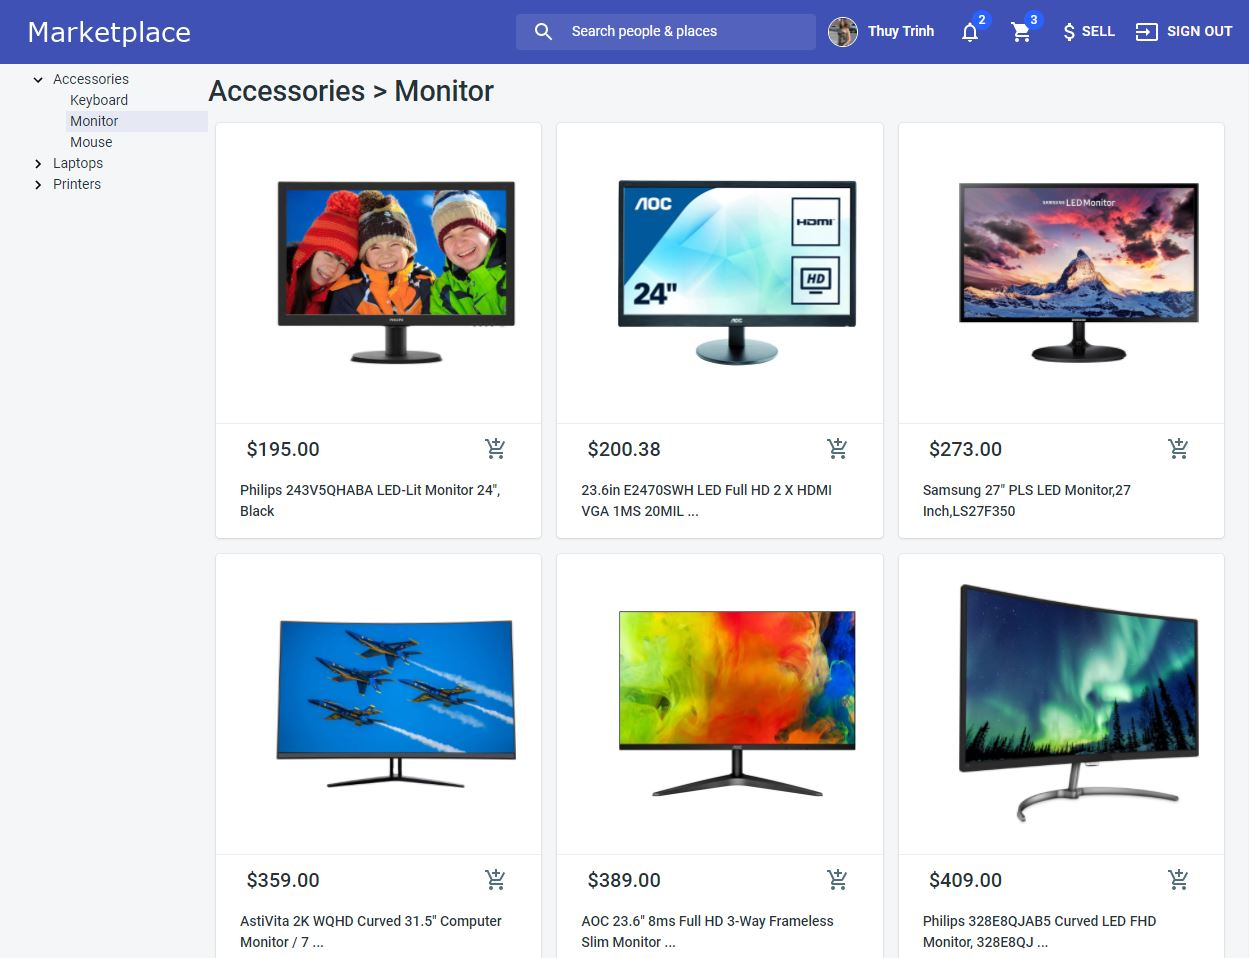
\includegraphics[width=3in]{images/marketplace_home.jpg}}
\end{figure}

\switchcolumn

\cvevent{}{Mr. Bill Mini Game}{May 2019}{\href{https://github.com/thuytrinhnguyen/mr-bill}{Source on GitHub}}
\begin{itemize}
	\item An under the sea themed mini game in which the character has to hit a set of balls into the basket using his hat while trying to avoid toxic eggs from the Jellyfish Boss
	\item Features:
	\subitem Cartoon design
	\subitem Life count
	\subitem Score count
	\subitem Gravity effect on balls
	\item Technologies: Processing 3.0 | Java
\end{itemize}

\begin{figure}[htbp]
	\centerline{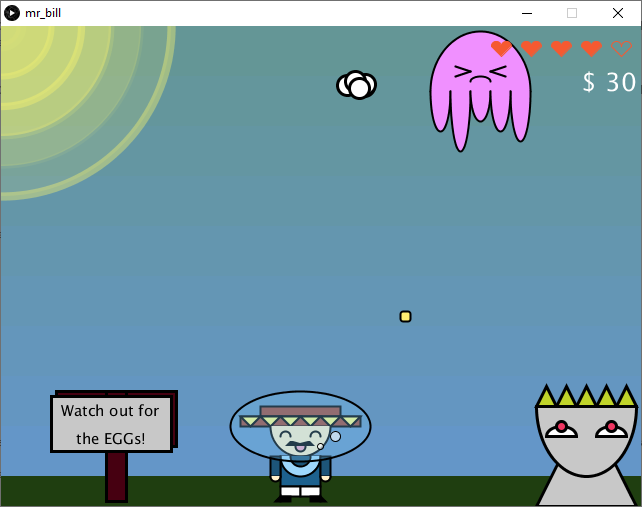
\includegraphics[width=3in]{images/mr-bill.png}}
\end{figure}

\switchcolumn

\divider

\cvevent{}{Statistics 270 - Linear Regression}{May 2019}{\href{https://github.com/thuytrinhnguyen/stat270-linear-regression}{Source on GitHub}}
\begin{itemize}
	\item Applying Linear Regression to predict the sea ice level of Atlantic Ocean
	\item Applying Multiple Linear Regression to identify how different factors affect wine quality
	\item Technologies: R | Markdown
\end{itemize}

\switchcolumn

\divider

\cvevent{}{This Resume}{Aug 2019}{\href{https://github.com/thuytrinhnguyen/cv}{Source on GitHub}}
\begin{itemize}
	\item This resume written in LaTeXs
	\item Technologies: TeXstudio | LaTeX
\end{itemize}

\end{paracol}

\newpage

\cvsection{Certificates}

\columnratio{0.5}

\begin{paracol}{2}

\cvevent{ Structuring Machine Learning Projects}{deeplearning.ai}{Aug 2020}{\href{https://www.coursera.org/account/accomplishments/certificate/7ZKGBX9AZDML}{Certificate}}

\divider

\cvevent{Improving Deep NNs: Hyperparameter tuning, Regularization and Optimization}{deeplearning.ai}{Aug 2020}{\href{https://www.coursera.org/account/accomplishments/certificate/6TXPN2QYUFNE}{Certificate}}

\divider

\cvevent{Neural Networks and Deep Learning}{deeplearning.ai}{Aug 2020}{\href{https://www.coursera.org/account/accomplishments/certificate/92TGPD88PLAQ}{Certificate}}

\divider

\cvevent{Maths for Machine Learning Specialization}{Imperial College London}{Aug 2020}{\href{https://www.coursera.org/account/accomplishments/specialization/certificate/WU7H7YWVSUGG}{Certificate}}

\divider

\cvevent{Maths for Machine Learning - PCA}{Imperial College London}{Aug 2020}{\href{https://www.coursera.org/account/accomplishments/certificate/Z9KCF2TGGDNF}{Certificate}}

\divider

\cvevent{Maths for Machine Learning - Linear Algebra}{Imperial College London}{Jul 2020}{\href{https://www.coursera.org/account/accomplishments/certificate/QYTL49D24C3L}{Certificate}}

\divider

\cvevent{Maths for Machine Learning - Calculus}{Imperial College London}{Jul 2020}{\href{https://www.coursera.org/account/accomplishments/certificate/5G93PV8NXBHK}{Certificate}}

\switchcolumn

\cvevent{Python for Data Science and AI}{IBM}{Jul 2020}{\href{https://www.coursera.org/account/accomplishments/certificate/AR7DAUH87HS4}{Certificate}}

\divider

\cvevent{Data Science Methodology}{IBM}{Sep 2019}{\href{https://www.coursera.org/account/accomplishments/verify/S9VR38XX8M9D}{Certificate}}

\divider

\cvevent{Tools for Data Science}{IBM}{Aug 2019}{\href{https://www.coursera.org/account/accomplishments/certificate/99JD2UZEST4H}{Certificate}}

\divider

\cvevent{What is Data Science?}{IBM}{Jul 2019}{\href{https://www.coursera.org/account/accomplishments/verify/D7HNBNBMLS3K}{Certificate}}

\divider

\cvevent{Basic Statistics}{University of Amsterdam}{Jun 2019}{\href{https://www.coursera.org/account/accomplishments/verify/AFENSVKYHZM8}{Certificate}}

\divider

\cvevent{Introduction to Typography}{California Institute of Arts}{Jun 2019}{\href{https://www.coursera.org/account/accomplishments/verify/AXUVQGT9L4NG}{Certificate}}

\divider

\cvevent{Fundamentals of Graphic Design}{California Institute of Arts}{Dec 2018}{\href{https://www.coursera.org/account/accomplishments/verify/DVW7YNPFHNW9}{Certificate}}

\end{paracol}

\vskip 0.2in

\cvsection{Extracurricular Activities}

\cvevent{Technical Advisor}{UAVS Start-up Challenge 2019}{Jun - Sep 2019}{Sydney}
\begin{itemize}
	\item Structured the 3-round format and rubrics with {\href{https://svf.org.vn/}{Start-up Vietnam Foundation}} 
	\item Planned a Lean Canvas training workshop for 80+ attendees
	\item Prepared sets of case studies and Q\&A questions for the Finale whose total prize worths \$10,000
\end{itemize}

\divider

\cvevent{Student Support Department - Media Teamlead}{The United Associations of Vietnamese Students in New South Wales}{Mar - Sep 2019}{Sydney}
\begin{itemize}
	\item Managed a 5-member team to deliver inforgraphics and videos every week for 03 months 
	\item Increased the organization Facebook group size by 600+ members/05 months
	\item Wrote script and directed a {\href{https://www.facebook.com/uavsnsw/videos/433640800560301/}{start-up motivational video}} with 2,000+ views
\end{itemize}

\cvevent{Intern Leader}{Tien Thinh Immigration Company}{Nov 2018 - Feb 2019}{Sydney}
\begin{itemize}
	\item Allocated tasks and supervised a 5-member group of interns
	\item Conducted a system proposal for an Asian Supermarket project (POS, accounting software, etc.)
\end{itemize}

\divider

\cvevent{Teamlead}{Global Volunteering Day 2018}{Mar - Jun 2018}{Vietnam}
\begin{itemize}
	\item Participated with 1,000+ participants from 30+ countries
	\item Hosted Mexican booth serving F\&B and games for 500+ participants
\end{itemize}

\divider

\cvevent{External Relations Intern}{Foreign Trade University - Incubator}{Jul 2017 - Jan 2018}{Vietnam}
\begin{itemize}
	\item Maintained and developed national and international partnership with 10+ partners
	\item Built a masterplan for the Incubator Japan and Korea training trips 
\end{itemize}

\divider

\cvevent{Vietnamese Representative}{APEC Youth Forum - Voices of the Future}{Sep - Nov 2017}{Vietnam}
\begin{itemize}
	\item Contributed to APEC Youth Declaration with 20 nation representatives
	\item Actively contributed to 05 conferences during APEC Leader's Week
\end{itemize}

\divider

\cvevent{External Relations Officer}{Tomorrow Entrepreneur Club - Foreign Trade University}{Oct 2015 - Jul 2017}{Vietnam}
\begin{itemize}
	\item Maintained and developed partnership with 20+ key partners
	\item Prepared 15+ reports for weekly meetings
	\item Liaised with 50+ enterprise partners and business people over the years
\end{itemize}

\end{document}
